% This file was created with tikzplotlib v0.10.1.
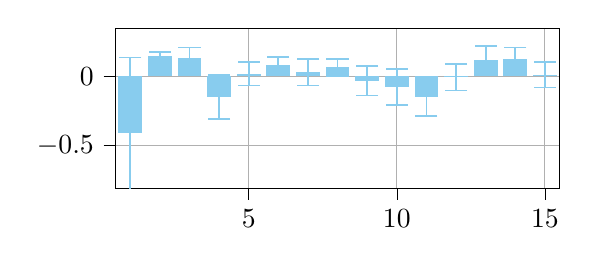
\begin{tikzpicture}

\definecolor{darkgray176}{RGB}{176,176,176}
\definecolor{skyblue136204238}{RGB}{136,204,238}

\begin{axis}[
height=1.4222438079424382in,
tick align=outside,
tick pos=left,
width=2.8444876158848764in,
x grid style={darkgray176},
xmajorgrids,
xmin=0.5, xmax=15.5,
xtick style={color=black},
y grid style={darkgray176},
ymajorgrids,
ymin=-0.80671120352567, ymax=0.347156413211247,
ytick style={color=black}
]
\draw[draw=none,fill=skyblue136204238] (axis cs:0.6,0) rectangle (axis cs:1.4,-0.40671120352567);
\draw[draw=none,fill=skyblue136204238] (axis cs:1.6,0) rectangle (axis cs:2.4,0.147156413211247);
\draw[draw=none,fill=skyblue136204238] (axis cs:2.6,0) rectangle (axis cs:3.4,0.134143424812531);
\draw[draw=none,fill=skyblue136204238] (axis cs:3.6,0) rectangle (axis cs:4.4,-0.148985896559106);
\draw[draw=none,fill=skyblue136204238] (axis cs:4.6,0) rectangle (axis cs:5.4,0.0193952704493765);
\draw[draw=none,fill=skyblue136204238] (axis cs:5.6,0) rectangle (axis cs:6.4,0.0786878259558603);
\draw[draw=none,fill=skyblue136204238] (axis cs:6.6,0) rectangle (axis cs:7.4,0.0291664689357056);
\draw[draw=none,fill=skyblue136204238] (axis cs:7.6,0) rectangle (axis cs:8.4,0.0646985965370845);
\draw[draw=none,fill=skyblue136204238] (axis cs:8.6,0) rectangle (axis cs:9.4,-0.0320907787931394);
\draw[draw=none,fill=skyblue136204238] (axis cs:9.6,0) rectangle (axis cs:10.4,-0.0769997034776862);
\draw[draw=none,fill=skyblue136204238] (axis cs:10.6,0) rectangle (axis cs:11.4,-0.150578656522061);
\draw[draw=none,fill=skyblue136204238] (axis cs:11.6,0) rectangle (axis cs:12.4,-0.00638258227143016);
\draw[draw=none,fill=skyblue136204238] (axis cs:12.6,0) rectangle (axis cs:13.4,0.117520190902406);
\draw[draw=none,fill=skyblue136204238] (axis cs:13.6,0) rectangle (axis cs:14.4,0.123687482998796);
\draw[draw=none,fill=skyblue136204238] (axis cs:14.6,0) rectangle (axis cs:15.4,0.0107010561742237);
\path [draw=skyblue136204238, semithick]
(axis cs:1,-0.949606239387161)
--(axis cs:1,0.13618383233582);

\path [draw=skyblue136204238, semithick]
(axis cs:2,0.11780288460071)
--(axis cs:2,0.176509941821783);

\path [draw=skyblue136204238, semithick]
(axis cs:3,0.059741019145157)
--(axis cs:3,0.208545830479906);

\path [draw=skyblue136204238, semithick]
(axis cs:4,-0.30606338508072)
--(axis cs:4,0.00809159196250858);

\path [draw=skyblue136204238, semithick]
(axis cs:5,-0.0662659928690008)
--(axis cs:5,0.105056533767754);

\path [draw=skyblue136204238, semithick]
(axis cs:6,0.0167882211376429)
--(axis cs:6,0.140587430774078);

\path [draw=skyblue136204238, semithick]
(axis cs:7,-0.0670037468872563)
--(axis cs:7,0.125336684758668);

\path [draw=skyblue136204238, semithick]
(axis cs:8,0.00307821788376025)
--(axis cs:8,0.126318975190409);

\path [draw=skyblue136204238, semithick]
(axis cs:9,-0.138188713352731)
--(axis cs:9,0.0740071557664519);

\path [draw=skyblue136204238, semithick]
(axis cs:10,-0.208240238975898)
--(axis cs:10,0.0542408320205255);

\path [draw=skyblue136204238, semithick]
(axis cs:11,-0.284861551618899)
--(axis cs:11,-0.0162957614252226);

\path [draw=skyblue136204238, semithick]
(axis cs:12,-0.102127204732227)
--(axis cs:12,0.0893620401893671);

\path [draw=skyblue136204238, semithick]
(axis cs:13,0.0175774172424872)
--(axis cs:13,0.217462964562325);

\path [draw=skyblue136204238, semithick]
(axis cs:14,0.0390944870456528)
--(axis cs:14,0.20828047895194);

\path [draw=skyblue136204238, semithick]
(axis cs:15,-0.0815476087439342)
--(axis cs:15,0.102949721092382);

\addplot [semithick, skyblue136204238, mark=-, mark size=4, mark options={solid}, only marks]
table {%
1 -0.949606239387161
2 0.11780288460071
3 0.059741019145157
4 -0.30606338508072
5 -0.0662659928690008
6 0.0167882211376429
7 -0.0670037468872563
8 0.00307821788376025
9 -0.138188713352731
10 -0.208240238975898
11 -0.284861551618899
12 -0.102127204732227
13 0.0175774172424872
14 0.0390944870456528
15 -0.0815476087439342
};
\addplot [semithick, skyblue136204238, mark=-, mark size=4, mark options={solid}, only marks]
table {%
1 0.13618383233582
2 0.176509941821783
3 0.208545830479906
4 0.00809159196250858
5 0.105056533767754
6 0.140587430774078
7 0.125336684758668
8 0.126318975190409
9 0.0740071557664519
10 0.0542408320205255
11 -0.0162957614252226
12 0.0893620401893671
13 0.217462964562325
14 0.20828047895194
15 0.102949721092382
};
\end{axis}

\end{tikzpicture}
